% \documentclass[12pt, twoside]{article}
\usepackage[letterpaper, margin=1in, headsep=0.2in]{geometry}
\setlength{\headheight}{0.6in}
%\usepackage[english]{babel}
\usepackage[utf8]{inputenc}
\usepackage{microtype}
\usepackage{amsmath}
\usepackage{amssymb}
%\usepackage{amsfonts}
\usepackage[nomessages]{fp} %\FPeval{\var-name}{2*sin(pi/6)}
\usepackage{siunitx} %units in math. eg 20\milli\meter
\usepackage{yhmath} % for arcs, overparenth command
\usepackage{tikz} %graphics
\usetikzlibrary{quotes, angles, arrows, arrows.meta}
\usepackage{graphicx} %consider setting \graphicspath{{images/}}
\usepackage{parskip} %no paragraph indent
\usepackage{enumitem}
\usepackage{multicol}
\usepackage{venndiagram}

\usepackage{fancyhdr}
\pagestyle{fancy}
\fancyhf{}
\renewcommand{\headrulewidth}{0pt} % disable the underline of the header
\raggedbottom
\hfuzz=2mm %suppresses overfull box warnings

\usepackage{hyperref}

\fancyhead[LE]{\thepage}
\fancyhead[RO]{\thepage \\ Name: \hspace{4cm} \,\\}
\fancyhead[LO]{BECA / Dr. Huson / Geometry\\*  Unit 11: Circle angles, sectors, arcs \\* 28 February 2023}

\begin{document}

\subsubsection*{11.2 Classwork: Sector area}
\begin{enumerate}
\item Lesson: Given circle $O$ with points on the circle $A$, $B$, $C$, $D$, $E$.
    \begin{multicols}{2}
    \raggedcolumns
    \begin{enumerate}[itemsep=0.5cm]
      \item Highlight the two radii $\overline{OD}$ and $\overline{OE}$
      \item The segments $\overline{AB}$ and $\overline{AC}$ are called \emph{chords} (pronounced with a hard ``c'', \emph{kord})
      \item The angle with the circle's center as its vertex is called a \emph{central angle}, $\angle DOE$
      \item The angle with its vertex on the circle is called an \emph{inscribed angle}, $\angle BAC$
      
    \end{enumerate}
    \begin{tikzpicture}[scale=0.8]
      \draw (0,0) circle[radius=4];
      \draw [thick]
      (0:4) node[above left] {$D$}--
      (0,0) node[left] {$O$}--
      (-60:4) node[below right] {$E$};
      \draw [thick]
      (120:4) node[above left] {$B$}--
      (200:4) node[left] {$A$}--
      (50:4) node[above right] {$C$};
      \node at (0,0) {$\bullet$};
    \end{tikzpicture}
    \end{multicols}

\item Highlight elements in circle $O$ with the required colors.
    \begin{multicols}{2}
    \raggedcolumns
    \begin{enumerate}[itemsep=0.5cm]
      \item The chords in yellow
      \item The diameter in red
      \item The vertex of the inscribed angle in blue
      \item What is the measure of the central angle, $\angle DOG$?
    \end{enumerate}
    \begin{tikzpicture}[scale=0.8]
      \draw (0,0) circle[radius=4];
      \draw [thick]
      (130:4) node[above left] {$G$}--
      (0,0) node[below left] {$O$}--
      (-50:4) node[below right] {$D$};
      \draw [thick]
      (120:4) node[above] {$A$}--
      (50:4) node[above right] {$B$}--
      (-20:4) node[right] {$C$};
      \draw [thick]
      (275:4) node[below] {$E$}--
      (165:4) node[left] {$F$};
      \node at (0,0) {$\bullet$};
    \end{tikzpicture}
    \end{multicols}

\item Given circle $O$ with points on the circle $A$, $B$, $C$, $D$ as shown. Find each central angle measure.
\begin{multicols}{2}
  \begin{enumerate} 
    \item $m\angle AOB =$
    \item $m\angle BOC =$
    \item $m\angle AOC =$
    \item What is the measure of the \emph{reflex angle} $m\angle AOC =$, i.e. the one containing point $D$ that is $>180^\circ$
    \end{enumerate}
\columnbreak
    \includegraphics[width=7.5cm]{../graphics/11central_angles.png}
    https://www.geogebra.org/calculator/xqketuwj
\end{multicols}

\newpage
\subsubsection*{Mixed review}
\item Given $A(-1,2)$ and $B(3,5)$, find the length of $\overline{AB}$. Show the substitution into the distance formula.
  %https://graspablemath.com/canvas?load=_024bda2a5587c074

\item Find the volume of a pyramid ($V=\frac{1}{3}Bh$) having a height of 11.3 inches and with a square base having side lengths of 7 inches. Express your result to the \emph{nearest cubic inch}. \vspace{5cm}

\item Find the volume of a hemisphere with a radius of 30 inches, to the \emph{nearest whole cubic inch}. (The formula for the volume of a \emph{sphere} is $V=\frac{4}{3}\pi r^3$ and a \emph{hemisphere} is half of a sphere.) \vspace{5cm}

\end{enumerate}
\end{document}
